\section{Decomposition 1: SIoTIP System (Av3, P2, UC11, UC14, UC15, UC18)}
\subsection{Module to decompose}
    In this run we decompose the \texttt{SIoTIP System}.

\subsection{Selected architectural drivers}
    The non-functional drivers for this decomposition are:
    \begin{itemize}
    	\item \emph{Av3}: Pluggable device or mote failure
    	\item \emph{P2}: Requests to the pluggable data database
    \end{itemize}

    \noindent The related functional drivers are:
    \begin{itemize}
        \item \emph{UC11}: Send pluggable device data (P2) \\
              This use case stores pluggable device data in the pluggable device data storage.
              This could be a sensor reading, or an actuator status.
    	\item \emph{UC14}: Send heartbeat (Av3) \\
              This use case checks whether or not motes and pluggable devices
              are still operational.
    	\item \emph{UC15}: Send notification (Av3) \\
              This use case sends a notification to a registered user.
    	\item \emph{UC18}: Check and deactivate applications (Av3) \\
              This use case deactivates any application that requires deactivation,
              because of unavailability of essential pluggable devices
              or unassigned mandatory roles.
    \end{itemize}

    \paragraph{Rationale}
    We chose Av3 first since it had high priority and it was more relevant to
    the core of the system (pluggable device data) than attributes M1 and U2. We
    chose P2 along with Av3 as it would force us to think about the way
    sensor data is handled. We believe this combination of pluggable device connectivity and
    storage of sensor data is the most defining feature of the system, and that
    handling this combination would give a better starting point than M1+U2
    for later ADD iterations.


\subsection{Architectural design}
    \paragraph{Application redundancy settings for Av3}
    Discussion of the solution selected for (a part of) one of the architectural
    drivers.

    \paragraph{Failure detection for Av3}
    timers? \\
    heartbeat/timestamp tactic

    \paragraph{Application deactivation for Av3}
    same as Application redundancy settings for Av3? \\
    degradation/removal from service tactic

    \paragraph{Notifications for Av3}
    from application manager to cust orgs and apps \\
    from gateway to infr owners \\
    notifications tactic

    \paragraph{Scheduling for P2}
    dynamic priority scheduling \\
    tactics: schedule resource, prioritize events, also limit event response?\\
    starvation avoidance \\
    \textit{TODO ASK: The  system  checks  whether  the  pluggable  device
    has  been  initialised (cf. UC8: Initialise  a pluggable device)}

    \paragraph{Pluggable data separation for P2}
    "pluggable data has no impact on other data"
    two databases


\subsubsection{Alternatives considered}
    \paragraph{Alternatives for X}
    A discussion of the alternative solutions and why that were not selected.


\subsection{Instantiation and allocation of functionality}
    \paragraph{Decomposition}
    Main aspects of the resulting decomposition.

    \subparagraph{ApplicationManager}
    deactivate apps
    ???? check mandatory user roles
    set redundancy in the available pluggable devices
    If application suspended or re-activated, notify cust. org.
    If application uses failed plugg device, notify application
    (Av3)

    \subparagraph{Database}
    General database for other data. Storage of notifications for now.

    \subparagraph{GatewayFacade}
    receive heartbeats, send heartbeats/device lists, send application shutdown, send notification trigger (Av3)\\
    forward data to applications

    \subparagraph{MoteFacade}
    sends heartbeats

    \subparagraph{NotificationHandler}
    Send notifications. \\
    stored by system \(->\) contact DB? \\
    lookup communication channel \\
    users choose delivery method?

    \subparagraph{PluggableDeviceDB}
    store data related to pluggable devices

    \subparagraph{PluggableDeviceFacade}
    send heartbeats

    \subparagraph{PluggableDeviceManager}
    check list of devices and see if there are pluggable devices for applications
    check redundancy in the available pluggable devices
    contains application preferences (e.g. amount of sensors required)
    can send command to deactivate application
    If failure detected, notify inf owner (Av3).
    reactivate application if new/needed hardware detected

    \subparagraph{PluggableDeviceDataScheduler}
    scheduling, detect overload mode, store data, forward data

    \begin{figure}[!htp]
    	\centering
    	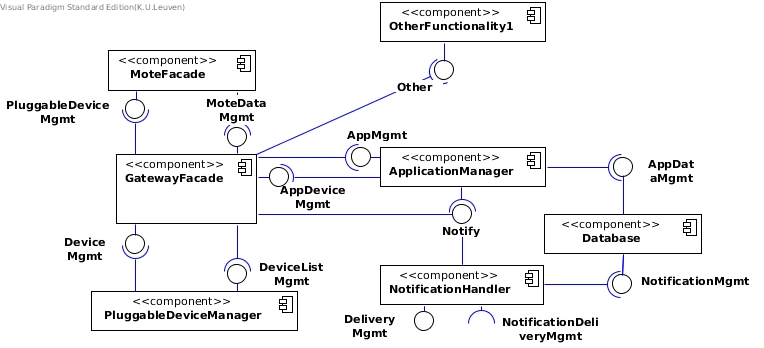
\includegraphics[width=0.8\textwidth]{component-diagram-1}
    	\caption{Component-and-connector diagram of this decomposition.}
        \label{fig:it1-cc_main}
    \end{figure}

% A SEQUENCE DIAGRAM FOR UC11 WOULD BE ACTUALLY VERY USEFUL (shows how the gateway checks if devices are initialised), 14 too: shows how applications can get deactivated
% REMOVE THIS PART BECAUSE MONEYKA IS LAAAAZZZZYYYYYY BAD STUDENT "IT IS NOT NECESSARY"
    % \paragraph{Behaviour}
    % If needed and explanation of the behaviour of certain aspects of the design so
    % far.

    % \begin{figure}[!htp]
    % 	\centering
    % 	%\includegraphics[width=0.8\textwidth]{}
    % 	\missingfigure[figwidth=0.8\textwidth]{Sequence diagram}
    % 	\caption{Sequence diagram illustrating a key behavioural aspect.
    % 	}\label{fig:it1-seq_aspect1}
    % \end{figure}

    \paragraph{Deployment}
    Rationale of the allocation of components to physical nodes.

    \begin{figure}[!htp]
    	\centering
    	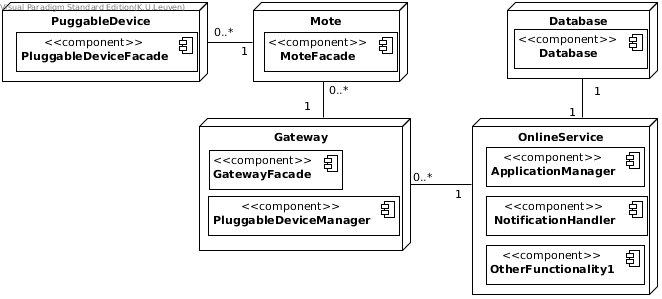
\includegraphics[width=0.8\textwidth]{deployment-diagram-1}
    	\caption{Deployment diagram of this decomposition.
    	}\label{fig:it1-depl_main}
    \end{figure}


\subsection{Interfaces for child modules}
    \subsubsection{ApplicationManager}
    \begin{itemize}
        \item ForwardData
        \begin{itemize}
            \item \texttt{void sendData(PluggableDeviceData data)}
            \begin{itemize}
                \item Effect: Send pluggable device data to an application that wants to use it
                \item Exceptions: None
            \end{itemize}
        \end{itemize}
        \item AppMgmt
        \begin{itemize}
            \item \texttt{void deactivateApplicationInstance(int applicationInstanceID)}
            \begin{itemize}
                \item Effect: Deactivates a running instance of an application.
                \item Exceptions: None
            \end{itemize}
            \item \texttt{void activateApplicationInstance(int applicationInstanceID)}
            \begin{itemize}
                \item Effect: Activates a new instance of an application.
                \item Exceptions: None
            \end{itemize}
        \end{itemize}
    \end{itemize}

    \subsubsection{Database}
    \begin{itemize}
        \item NotificationMgmt
        \begin{itemize}
            \item \texttt{int storeNotification(NotificationData data)}
            \begin{itemize}
                \item Effect: Stores a new notification entry in the database. Returns the id of the new notification.
                \item Exceptions: None
            \end{itemize}
            \item \texttt{void updateNotification(NotificationData data)}
            \begin{itemize}
                \item Effect: Updates an existing notification (e.g. change status to "sent").
                \item Exceptions: None
            \end{itemize}
            \item \texttt{int lookupNotificationChannelForUser(int userID)}
            \begin{itemize}
                \item Effect: Returns the type of communication channel a user prefers.
                              Different communication channels are mapped to integers.
                \item Exceptions: None
            \end{itemize}
        \end{itemize}
        \item AppDataMgmt
        \begin{itemize}
            \item \texttt{void updateApplication(ApplicationData data)}
            \begin{itemize}
                \item Effect: Updates an application in the database (e.g. change state to 'inactive').
                \item Exceptions: None
            \end{itemize}
            \item \texttt{void updateSubscription(SubscriptionData data)}
            \begin{itemize}
                \item Effect: Updates a subscription in the database (e.g. change state to 'disabled').
                \item Exceptions: None
            \end{itemize}
        \end{itemize}
    \end{itemize}

    \subsubsection{GatewayFacade}
    \begin{itemize}
        \item MoteDataMgmt
        \begin{itemize}
            \item \texttt{void sendHeartbeat(int moteID, List<PluggableDeviceInfo> devices)}
            \begin{itemize}
                \item Effect: Sends a heartbeat to a certain gateway with information about operational devices.
                \item Exceptions: None
            \end{itemize}
            \item \texttt{void sendData(PluggableDeviceData data)}
            \begin{itemize}
                \item Effect: Sends pluggable device data to the connected mote.
                \item Exceptions: None
            \end{itemize}
        \end{itemize}
        \item DeviceMgmt
        \begin{itemize}
            \item \texttt{void initialiseDevice(int deviceID, PluggableDeviceSettings settings)}
            \begin{itemize}
                \item Effect: Initialises a pluggable device for use with the system. TODO check QA's text
                \item Exceptions: None
            \end{itemize}
            \item \texttt{List<DeviceInfo> getConnectedDevices()}
            \begin{itemize}
                \item Effect: Describe the effect of calling this operation.
                \item Exceptions: None
            \end{itemize}
            \item \texttt{void timerExpired(int deviceID)}
            \begin{itemize}
                \item Effect: Lets the gateway know that a timer for pluggable device or mote has expired.
                              This will generate a notification for an infrastructure owner.
                \item Exceptions: None
            \end{itemize}
            \item \texttt{void deactivateApplicationInstance(int applicationInstanceID)}
            \begin{itemize}
                \item Effect: Deactivates a certain application. This could happen when
                              mandatory pluggable devices for the application are missing.
                \item Exceptions: None
            \end{itemize}
            \item \texttt{void reactivateApplicationInstance(int applicationInstanceID)}
            \begin{itemize}
                \item Effect: Reactivate an application instance. This could happen
                              automatically after a broken sensor has been replaced.
                \item Exceptions: None
            \end{itemize}
        \end{itemize}
        \item CheckDevices
        \begin{itemize}
            \item \texttt{bool areEssentialDevicesOperational(int applicationID)}
            \begin{itemize}
                \item Effect: Returns true if all essential devices for the application
                              with id "applicationID" are operational.
                \item Exceptions: None
            \end{itemize}
        \end{itemize}
    \end{itemize}

    \subsubsection{MoteFacade}
    \begin{itemize}
        \item PluggableDeviceDataMgmt
        \begin{itemize}
            \item \texttt{void sendData(PluggableDeviceData data)}
            \begin{itemize}
                \item Effect: Sends pluggable device data to the connected mote.
                \item Exceptions: None
            \end{itemize}
            \item \texttt{List<DeviceInfo> getConnectedDevices()}
            \begin{itemize}
                \item Effect: Returns a list of information about devices that are connected to the mote.
                \item Exceptions: None
            \end{itemize}
        \end{itemize}

        \item PluggableDeviceMgmt
        \begin{itemize}
            \item \texttt{void initialise(int deviceID, PluggableDeviceSettings settings)}
            \begin{itemize}
                \item Effect: TODO check this with QA's: Initialises a connected pluggable device according to some settings
                \item Exceptions: None
            \end{itemize}
        \end{itemize}
    \end{itemize}

    \subsubsection{NotificationHandler}
    \begin{itemize}
        \item Notify
        \begin{itemize}
            \item \texttt{void notify(int userID, String message)}
            \begin{itemize}
                \item Effect: Describe the effect of calling this operation.
                \item Exceptions: None
            \end{itemize}
        \end{itemize}
        \item DeliveryMgmt
        \begin{itemize}
            \item \texttt{void sendAcknowledgement(int notificationID)}
            \begin{itemize}
                \item Effect: Sends an acknowledgement to the system for a certain notification.
                \item Exceptions: None
            \end{itemize}
        \end{itemize}
    \end{itemize}

    \subsubsection{External notification delivery serivce}
    \begin{itemize}
        \item NotificationDeliveryMgmt
        \begin{itemize}
            \item \texttt{void notify(JSONObject data)}
            \begin{itemize}
                \item Effect: Deliver a notification to an end user using a specific delivery service.
                \item Exceptions: None
            \end{itemize}
        \end{itemize}
    \end{itemize}

    \subsubsection{PluggableDeviceDB}
    \begin{itemize}
        \item PluggableDeviceDataMgmt
        \begin{itemize}
            \item \texttt{void sendData(PluggableDeviceData data)}
            \begin{itemize}
                \item Effect: Sends pluggable device data to the DB to be stored.
                \item Exceptions: None
            \end{itemize}
            \item \texttt{List<PluggableDeviceData> getData(int deviceID, DateTime from, DateTime to)}
            \begin{itemize}
                \item Effect: Returns data from a specific device in a certain time period.
                \item Exceptions: None
            \end{itemize}
            \item \texttt{List<int> getApplicationsForDevice(int deviceID)}
            \begin{itemize}
                \item Effect: Returns a list of applications that can use the device with id "deviceID."
                \item Exceptions: None
            \end{itemize}
        \end{itemize}
    \end{itemize}

    \subsubsection{PluggableDeviceFacade}
    \begin{itemize}
    	\item PluggableDeviceMgmt
    	\begin{itemize}
            \item \texttt{void initialise(PluggableDeviceSettings settings)}
            \begin{itemize}
                \item Effect: TODO check this with QA's: Initialises the pluggable device according to some settings
                \item Exceptions: None
            \end{itemize}
    	\end{itemize}
    \end{itemize}

    \subsubsection{PluggableDeviceManager}
    \begin{itemize}
    	\item DeviceListMgmt
    	\begin{itemize}
    		\item \texttt{void sendHeartbeat(int moteID, List<PluggableDeviceInfo> devices)}
    		\begin{itemize}
    			\item Effect: Send a heartbeat from a mote to check/update timers for operational devices.
    			\item Exceptions: None
    		\end{itemize}
    		\item \texttt{bool isDeviceInitialised(int deviceID)}
    		\begin{itemize}
    			\item Effect: Returns true if the device with id "deviceID" has been initialized.
    			\item Exceptions: None
    		\end{itemize}
    		\item \texttt{bool areEssentialDevicesOperational(int applicationID)}
    		\begin{itemize}
    			\item Effect: Returns true if all essential devices for the application
                              with id "applicationID" are operational.
    			\item Exceptions: None
    		\end{itemize}
    	\end{itemize}
    \end{itemize}

    \subsubsection{PluggableDeviceDataScheduler}
    \begin{itemize}
    	\item RequestData
    	\begin{itemize}
    		\item \texttt{List<PluggableDeviceData> requestData(int applicationID, int deviceID, DateTime from, DateTime to)}
    		\begin{itemize}
    			\item Effect: Request data from a specific device in a certain time period
    			\item Exceptions: None
    		\end{itemize}
    	\end{itemize}
    	\item PluggableDeviceDataMgmt
    	\begin{itemize}
    		\item \texttt{void sendData(PluggableDeviceData data)}
    		\begin{itemize}
    			\item Effect: Sends pluggable device data to the scheduler to be processed.
    			\item Exceptions: None
    		\end{itemize}
    	\end{itemize}
    \end{itemize}


\subsection{Data type definitions}
    \paragraph{PluggableDeviceData} contains data from a pluggable device at a certain point in time
                                    (e.g. a sensor reading, an actuator status)
    \paragraph{PluggableDeviceSettings} contains settings for a pluggable device (power status,
                                        data update rate, ...)
    \paragraph{PluggableDeviceInfo} contains information about a pluggable device (device id,
                                    power status, data update rate, ...)
    \paragraph{DateTime} Represents an instant in time, typically expressed as a date and time of day.

    \paragraph{NotificationData} contains data about a notification (message text, recipient,
                                 communication channel, date, status, source, ...).

    \paragraph{ApplicationData} contains data about an application instance (instance id, running status, ...)
    \paragraph{SubscriptionData} contains data about a subscription (subscription id, subscription status,
                                 subscription period, ...).


\subsection{Verify and refine}
    Completely handled: Av3, P2, UC11, UC14, UC15, UC18 \\

    \noindent This section describes per component which (parts of) the remaining
    requirements it is responsible for.

    \paragraph{ApplicationManager}
        \begin{itemize}
            \item  \emph{Av2}: Application failure \\
                   Prevention: a, b \\
                   Detection: a, b, c \\
                   Resolution: a, b, c
           \item \emph{P1}: Large number of users: c
           \item \emph{M1}: Integrate new sensor or actuator manufacturer: 1.c, 2.a
           \item \emph{M2}: Big data analytics on pluggable data and/or application usage data: d, e
           \item \emph{U1}: Application updates: a, b, c, d
           \item \emph{U2}: Easy Installation: e
           \item \emph{U12}: Perform actuation command
           \item \emph{UC17}: Activate an application: 3, 4
        \end{itemize}

    \paragraph{Database}
        \begin{itemize}
          	\item None
        \end{itemize}

    \paragraph{GatewayFacade}
        \begin{itemize}
            \item \emph{Av1}: Communication between SIoTIP gateway and Online Service \\
                               Resolution: b, c, d
            \item \emph{M1}: Integrate new sensor or actuator manufacturer: 1.a, 2.b
            \item \emph{U2}: Easy Installation: a, c, d
    \end{itemize}

    \paragraph{MoteFacade}
        \begin{itemize}
            \item \emph{M1}: Integrate new sensor or actuator manufacturer: 1.a, 2.b
            \item \emph{U2}: Easy Installation: b, c, d
            \item \emph{UC4}: Install mote: 1, 2
            \item \emph{UC5}: Uninstall mote: 1
            \item \emph{UC6}: Insert a pluggable device into a mote: 2
            \item \emph{UC7}: Remove a pluggable device from its mote: 2
        \end{itemize}

    \paragraph{NotificationHandler}
        \begin{itemize}
            \item \emph{UC16}: Consult notification message: 5
            \item \emph{UC17}: Activate an application: 5, 6
        \end{itemize}

    \paragraph{OtherFunctionality}
        \begin{itemize}
            \item \emph{Av1}: Communication between SIoTIP gateway and Online Service \\
                               Detection: a, b, c, d
                               Resolution: a
           	\item \emph{P1}: Large number of users: a
            \item \emph{M1}: Integrate new sensor or actuator manufacturer: 1.d
            \item \emph{M2}: Big data analytics on pluggable data and/or application usage data: a
            \item \emph{U2}: Easy Installation: e
            \item \emph{UC1}: Register a customer organisation
            \item \emph{UC2}: Register an end-user
            \item \emph{UC3}: Unregister an end user
            \item \emph{UC4}: Install mote: 3
            \item \emph{UC5}: Uninstall mote: 2.b
            \item \emph{UC6}: Insert a pluggable device into a mote: 3: topology part; alternative 3a.1.b
            \item \emph{UC7}: Remove a pluggable device from its mote: 3.b
            \item \emph{UC8}: Initialise a pluggable device: 1, 2, 4
            \item \emph{UC9}: Configure pluggable device access rights
            \item \emph{UC10}: Consult and configure the topology
            \item \emph{UC13}: Configure pluggable device
            \item \emph{UC16}: Consult notification message: 1, 2, 3, 4
            \item \emph{UC17}: Activate an application: 1, 2
            \item \emph{UC19}: Subscribe to application
            \item \emph{UC20}: Unsubscribe from application
            \item \emph{UC21}: Send invoice
            \item \emph{UC22}: Upload an application
            \item \emph{UC23}: Consult application statistics
            \item \emph{UC24}: Consult historical data
            \item \emph{UC25}: Access topology and available devices
            \item \emph{UC26}: Send application command or message to external front-end
            \item \emph{UC27}: Receive application command or message to external front-end
            \item \emph{UC28}: Log in
            \item \emph{UC29}: Log out
        \end{itemize}

    \paragraph{PluggableDeviceDB}
        \begin{itemize}
            \item \emph{M1}: Integrate new sensor or actuator manufacturer: 1.a, 1.b, 2.b
            \item \emph{M2}: Big data analytics on pluggable data and/or application usage data: b
        \end{itemize}

    \paragraph{PluggableDeviceFacade}
        \begin{itemize}
        	\item \emph{U2}: Easy Installation: d
        \end{itemize}

    \paragraph{PluggableDeviceManager}
        \begin{itemize}
            \item \emph{U2}: Easy Installation: c, d
            \item \emph{UC4}: Install mote: 4
            \item \emph{UC5}: Uninstall mote: 2
            \item \emph{UC6}: Insert a pluggable device into a mote: 3: uninitialised part; alternative 3a.1 3a.2 3a.4; 4
            \item \emph{UC7}: Remove a pluggable device from its mote: 3.a, 3.c
            \item \emph{UC8}: Initialise a pluggable device: 3,
        \end{itemize}

    \paragraph{PluggableDeviceDataScheduler}
        \begin{itemize}
            \item \emph{P1}: Large number of users: b
            \item \emph{M1}: Integrate new sensor or actuator manufacturer: 1.a, 2.b
            \item \emph{M2}: Big data analytics on pluggable data and/or application usage data: b, c
        \end{itemize}
